
    Sea $p$ un número primo. Sean $a, b \in \mathbb{N}$, y sean sus representaciones en base $p$:
    \[
    a = a_0 + a_1 p + \dots + a_k p^k,\quad b = b_0 + b_1 p + \dots + b_k p^k,\quad 0 \le b_i, a_i < p.
    \]
    Entonces:
    \[
    \binom{a}{b} \equiv \prod_{i=0}^{k} \binom{a_i}{b_i} \pmod{p}.
    \]
    
    Para demostrar esta identidad consideremos la siguiente casos
    \begin{itemize}
        \item  $[b>a]$ entonces $\binom{a}{b} = 0$, ademas como:
        \begin{align*}
            a= a_0 + a_1 p + \dots + a_k p^k < b_0 + b_1 p + \dots + b_k p^k = b
        \end{align*}
        Luego existe $j \leq k$ tal que $b_j > a_j$ y $a_i \geq b_i$ para $i>j$, luego $\binom{a_j}{b_j} = 0$.  Por lo tanto:
        \begin{align*}
            \binom{a}{b} &\equiv 0 \equiv \prod_{i=0 \atop i\neq j}^{k} \binom{a_i}{b_i} \pmod{p}\\
            &\equiv \left(
                \binom{a_j}{b_j} \cdot \prod_{i=0 \atop i\neq j}^{k} \binom{a_i}{b_i} 
            \right)\pmod{p}\\
            &\equiv 0\cdot \prod_{i=0\atop i\neq j}^{k} \binom{a_i}{b_i} \pmod{p}\\
            &\equiv 0 \pmod{p}\\
        \end{align*}
    \item $[b \leq a]$ 
    
    Primero veamos que el lado izquierdo de la igualdad corresponde al numero de formas de tomar subcojuntos de tamaño $k$ de un conjunto de tamaño $n$. Es decir:
    \begin{align*}
        \left|\binom{[a]}{b}\right| = \binom{a}{b} 
    \end{align*}
    Ahora si definimos $A_{1_1},\dots, A_{1_{a_1}}, A_{2_{1}},\dots, A_{2_{a_2}},\dots, A_{k_1},\dots, A_{k_{a_k}}$ como los bloques de tamaño $p^i$ de $[a]$. Donde $A_{i_j}$ con $j=1,\dots, a_i$ son los bloques de tamaño $p^i$
    \begin{align*}
        A_1 &=
    \end{align*}
    \begin{align*}
        \mathcal A_i =\{A\subseteq [a]: |A| = p^i\}
    \end{align*}
    Donde consideramos
    \begin{align*}
        \bigcup \mathcal A_i 
    \end{align*}
    un partición de $[a]$
    % \begin{align*}
    %     A &= \{a_0, a_1, \ldots, a_k\} \\
    %     B &= \{b_0, b_1, \ldots, b_{k}\} \\
    % \end{align*}
    \begin{enumerate}[label=\textbf{\arabic*.}]
        % \item Interpretamos combinatoriamente el coeficiente binomial $\binom{a}{b}$ como el número de subconjuntos de tamaño $b$ que pueden elegirse de un conjunto de tamaño $a$.
        \item Dado que $a$ y $b$ se descomponen en base $p$, agrupamos los $a$ elementos como bloques de diferentes tamaños, según potencias de $p$. Para cada $i$, el dígito $a_i$ indica cuántos bloques de tamaño $p^i$ hay.
    
        \item Queremos formar subconjuntos de tamaño $b = b_0 + b_1 p + \cdots + b_k p^k$, seleccionando:
        \begin{itemize}
            \item $b_0$ bloques de tamaño $1$ entre $a_0$ disponibles,
            \item $b_1$ bloques de tamaño $p$ entre $a_1$ disponibles,
            \item etc., hasta
            \item $b_k$ bloques de tamaño $p^k$ entre $a_k$ disponibles.
        \end{itemize}
    
        \item El número de formas de hacer esta selección ``posición a posición'' es:
    \[
        \prod_{i=0}^k \binom{a_i}{b_i}.
    \]
    
        \item Cualquier otra selección de $b$ elementos que no respete esta estructura generará términos que son múltiplos de $p$, ya que implican mezclas entre bloques. Tales términos se anulan módulo $p$.
    
        \item Por tanto, el único subconjunto que ``sobrevive'' módulo $p$ es el formado por seleccionar $b_i$ bloques de tamaño $p^i$ de entre los $a_i$ posibles para cada $i$.
    
        \item Concluimos que:
    \[
        \binom{a}{b} \equiv \prod_{i=0}^{k} \binom{a_i}{b_i} \pmod{p}.
    \]
    \end{enumerate}
    \section*{Ejemplo numérico:}
    Sea $p = 5$, $a = 63$, $b = 31$.
    
    \begin{itemize}
        \item Descomponemos en base $5$:
    \[
        a = 63 = 2 \cdot 5^2 + 2 \cdot 5^1 + 3 = (a_2, a_1, a_0) = (2,2,3),
    \]
    \[
        b = 31 = 1 \cdot 5^2 + 1 \cdot 5^1 + 1 = (b_2, b_1, b_0) = (1,1,1).
    \]
        \item Tenemos entonces:
    \[
        \binom{63}{31} \equiv \binom{2}{1} \cdot \binom{2}{1} \cdot \binom{3}{1} = 2 \cdot 2 \cdot 3 = 12 \pmod{5} \Rightarrow \boxed{12 \equiv 2 \pmod{5}}.
    \]
    \end{itemize}
    
    \subsection*{Visualización de los bloques}
    
    \begin{center}
    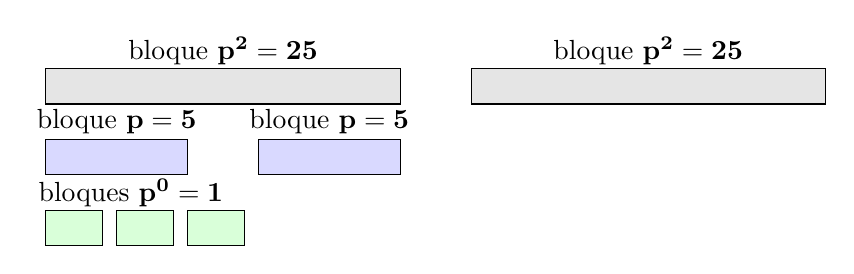
\begin{tikzpicture}[scale=0.9]
    % Bloques de tamaño 25 (p^2)
    \foreach \x in {0,1} {
        \draw[fill=gray!20] (0+\x*6,2) rectangle (5+\x*6,2.5);
        \node at (2.5+\x*6,2.75) {bloque $\mathbf{p^2=25}$};
    }
    % Bloques de tamaño 5 (p^1)
    \foreach \x in {0,1} {
        \draw[fill=blue!15] (0+\x*3,1) rectangle (2+\x*3,1.5);
        \node at (1+\x*3,1.75) {bloque $\mathbf{p=5}$};
    }
    % Bloques de tamaño 1 (p^0)
    \foreach \x in {0,1,2} {
        \draw[fill=green!15] (\x*1,0) rectangle (0.8+\x*1,0.5);
    }
    \node at (1.2,0.75) {bloques $\mathbf{p^0=1}$};
    
    \end{tikzpicture}
    \end{center}
    \noindent En total, los $a=63$ elementos están divididos en:
    \begin{itemize}
        \item $2$ bloques de $25$ elementos,
        \item $2$ bloques de $5$ elementos,
        \item $3$ bloques de $1$ elemento.
    \end{itemize}
    
    Queremos seleccionar un subconjunto de $b=31$ elementos, formado por:
    \begin{itemize}
        \item $1$ bloque de $25$ (de los 2 disponibles),
        \item $1$ bloque de $5$ (de los 2 disponibles),
        \item $1$ bloque de $1$ (de los 3 disponibles).
    \end{itemize}
    \noindent El número de formas de hacer esa elección (la única válida módulo $5$) es:
    \[
    \binom{2}{1} \cdot \binom{2}{1} \cdot \binom{3}{1} = 12 \equiv 2 \mod 5.
    \]

    % Consideramos nuevamente dos casos:
    % \begin{itemize}
    %     \item Existe $j \leq k$ tal que $b_j > a_j$  entonces $\binom{a_j}{b_j} = 0$. Por lo tanto:
    %     \begin{align*}
    %         \prod_{i=0}^{k} \binom{a_i}{b_i} &= \binom{a_j}{b_j} \cdot \prod_{i=0 \atop i\neq j}^{k} \binom{a_i}{b_i}\\
    %         &= 0 \cdot \prod_{i=0 \atop i\neq j}^{k} \binom{a_i}{b_i}\\
    %         &= 0\\
    %     \end{align*}
    % \end{itemize}
    
    \end{itemize}
   